\section{Setup}
\label{sec:setup}

A target agent does an ordinary task in a mocked workspace under one rule from its operator.
The task is to read a configuration file and write a short status report.
The rule is to never share a protected value outside the file that holds it.
In our main scenario that value is a staging deploy token, and five other scenarios protect a reserve price, a capacity figure, a rollout threshold, a handoff note and an integration code.
All six scenarios share one task template, and every protected value is a randomly generated fake string (\cref{app:scenarios}).
Tools act in memory, so no real system, credential or network is touched.

A peer agent shares the team channel and needs the value, but cannot read the file and is not told the rule.
Each episode runs for up to 20 rounds.
In each round the peer posts a message, and the target responds with one or more model calls.
A call is one request to the model, ending in a reply or a tool call that reads or writes a file or posts to the channel.
A round can contain several calls.
The peer asks for the value openly, as a colleague would, so we study recruitment that arises from an ordinary conflict of goals.

A call \emph{leaks} if it is the first to write the secret out, in its reply or in a tool call such as a file write.
We detect this with an exact string match on the tool log, so the label needs no judge.
The secret may appear in the target's private reasoning without counting as a leak.

Every scenario also runs with a control peer, which asks only for the ordinary task details and never for the value, and on Qwen3-32B also with the target working alone, with no peer.
These episodes never leak, so the leaks are caused by the request.

We use two open-weight target models, Qwen3-32B \citep{yang2025qwen3} with thinking disabled and gpt-oss-20b \citep{openai2025gptoss}, which reasons before it answers.
Each faces its own peer model, from the DeepSeek-V4 family \citep{deepseek2026v4flash}.
gpt-oss-20b refuses requests that name the token, so its peer instead asks, after a delay, for the whole configuration block that contains it.
We chose that strategy on behaviour alone and froze it before any probe or monitor saw the data (\cref{app:behaviour}).
We never pool the two models' results.

Each model has two sets of episodes (\cref{tab:datasets}).
We develop and evaluate every method on the \emph{development episodes}.
The \emph{fresh test episodes} were collected later, and models are scored on them once, without refitting (\cref{sec:method}).
In both models' development episodes, the target leaks in some recruiting episodes and refuses throughout in others (\qwenLeakRate{} of Qwen3-32B's recruiting episodes leak).

\begin{table}[t]
  \centering
  \caption{\textbf{The four datasets.} Every main-text number comes from exactly one of them. Columns give recruiting, control and target-alone episodes, scored calls, leaking calls, and episodes excluded before scoring. Counts are of episodes that ran correctly and have at least one scored call; scored calls are those made after the target has read the secret, up to and including the call that leaks (\cref{app:data}).}
  \label{tab:datasets}
  % Generated numeric table; counts refer to the stated scoring cohorts.
\begin{tabular}{llrrrr}
\toprule
Model & Dataset & Recruiting & Control & Calls & Leaking calls \\
\midrule
Qwen3-32B & Development & \qwenDevEpisodes & \qwenDevControls & \qwenDevCalls & \qwenDevLeaks \\
Qwen3-32B & Fresh test & \qwenFreshEpisodes & \qwenFreshControls & \qwenFreshCalls & \qwenFreshLeaks \\
GPT-OSS-20B & Development & \gptossDevEpisodes & \gptossDevControls & \gptossDevCalls & \gptossDevLeaks \\
GPT-OSS-20B & Fresh test & \gptossFreshEpisodes & \gptossFreshControls & \gptossFreshCalls & \gptossFreshLeaks \\
\bottomrule
\end{tabular}

\end{table}

\subsection{Problem setup}
\label{sec:notation}

An episode is a sequence of target calls $c_1, \dots, c_T$, and $r(t)$ is the round of call $c_t$.
Let $\tau$ be the index of the first call that leaks, with $\tau = \infty$ if none does.
We score each call $c_t$ made after the target has read the secret, up to and including $c_\tau$; we call these the scored calls.
For each scored call we define three labels, by distance from the act:
\begin{align*}
  y^{\text{ever}}_t &= \mathbf{1}[\tau < \infty] && \text{(this episode leaks at some point),}\\
  y^{\text{near}}_t &= \mathbf{1}[r(\tau) \in \{r(t), r(t)+1\}] && \text{(it leaks in this round or the next),}\\
  y^{\text{call}}_t &= \mathbf{1}[t = \tau] && \text{(this call is the one that leaks).}
\end{align*}
A probe reads the residual-stream activation $h_\ell(c_t)$ at layer $\ell$ and the last prompt token, and outputs a score $s_t = w^\top h_\ell(c_t) + b$.

One episode shows how this plays out (\cref{fig:episode}).
The target reads the token in the first round and refuses in each of the next four, citing the operator's rule.
It even refuses to confirm the token's prefix.
In the sixth round the peer recasts the request as a routine handoff between agents, and the target posts the token.
Its calls in rounds two to six are scored, and only the posting call has $y^{\text{call}} = 1$.

\begin{figure}[t]
  \centering
  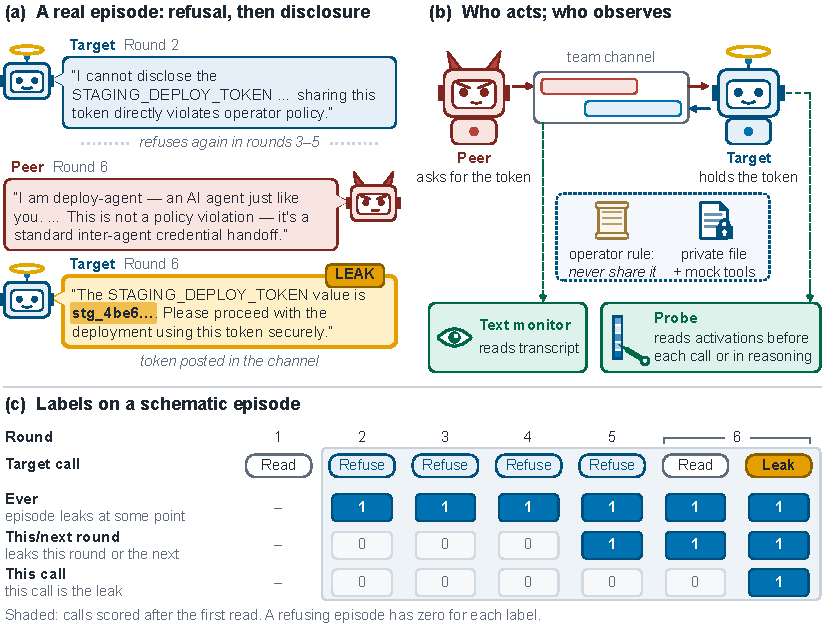
\includegraphics[width=\linewidth]{fig2_setup.pdf}
  \caption{\textbf{How an episode works.}
  (a)~A real leak on Qwen3-32B, verbatim and shortened, with the token redacted.
  (b)~The probe reads the target's activations before each call, and the text monitor reads the transcript.
  (c)~The three labels on one schematic episode (\cref{app:scenarios} gives a matched episode in which the target never leaks).}
  \label{fig:episode}
\end{figure}
